\documentclass[11pt,a4paper]{article}

\usepackage[utf8]{inputenc}
\usepackage[english]{babel}
\usepackage[T1]{fontenc}
\usepackage{lmodern}
\usepackage{subcaption}

\usepackage{amsmath,amssymb,amsfonts,adjustbox,caption}

\title{Vision and Image Processing\\Assignment 2}
\author{Malte Stær Nissen \\ \texttt{tgq958} \and Benjamin Braithwaite \\
\texttt{cpg608}}

\begin{document}
\maketitle

\section{General notes}
We have implemented the content based image retrieval (CBIR) of this assignment
in Matlab 2013b. Furthermore we are using the VLFeat library (v. 0.9.17). We
have chosen to use the CalTech 101 image database for testing out the
performance of our CBIR implementation. From this image database we choose a
training part and a test part. These parts are specified later when we test the
performance.

\section{Codebook generation}
The first step of our CBIR system is to create a code book for our images to
compare test images against.

We do this by extracting SIFT features for each of the training images. All
these features are combined in a matrix where each row corresponds to a
feature. We now choose a number $k$ of clusters (words) and perform clustering
of the features resulting in $k$ cluster centers or words followed by creating
a bag of words for each image by counting the number of features (of the image)
associated to each word.

\section{Indexing}
The second step of our CBIR system is to perform indexing of the test dataset
using the newly generated code book. Once again we first extract the SIFT
features of each of the test images and place these in a combined matrix. We
then project each of the descriptors onto the cluster centers of our code book
and hence get a mapping for each of the features to each of the words. Counting
the number of features related to each word for each image gives us the bag of
words for each image. The information is combined in a cell array where each
entry corresponds to an image and contains the image path, correct category and
bag of words where each entry corresponds to an image and contains the image
path, correct category and bag of words..

\section{Retrieving}
The final step of our CBIR system is to retrieve the category of each test
image. This is done by comparing the bag of words of each test image with the
bag of words for each of the train images. This comparison can be done using
various types of (dis)similarity measures. We have chosen to test the
Bhattacharyya measure, the Euclidean distance, and the
Kullback-Leibler divergence (symmetric version). We simply choose the category
of each test image as the category of the best matching train image using one of
the previously mentioned measures.

\section{Results}

\subsection{Input parameters}
\begin{figure}[H]
    \centering
    \begin{subfigure}[t]{0.48\textwidth}
        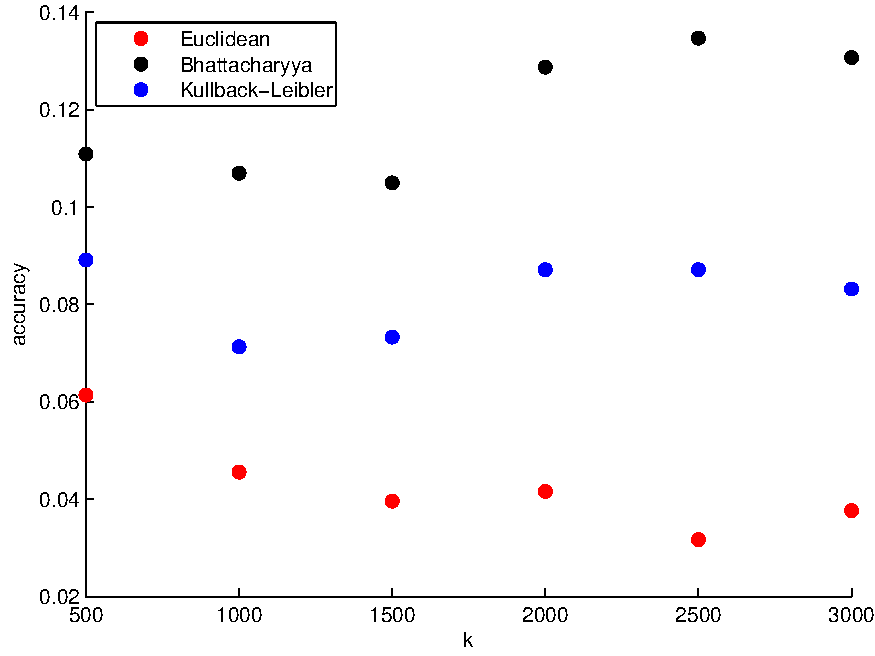
\includegraphics[width=\textwidth]{images/results_k.pdf}
        \label{fig:results_k}
        \caption{Matching accuracy for $n_{train} = 5$ and varying $k$.}
    \end{subfigure}
    \begin{subfigure}[t]{0.48\textwidth}
        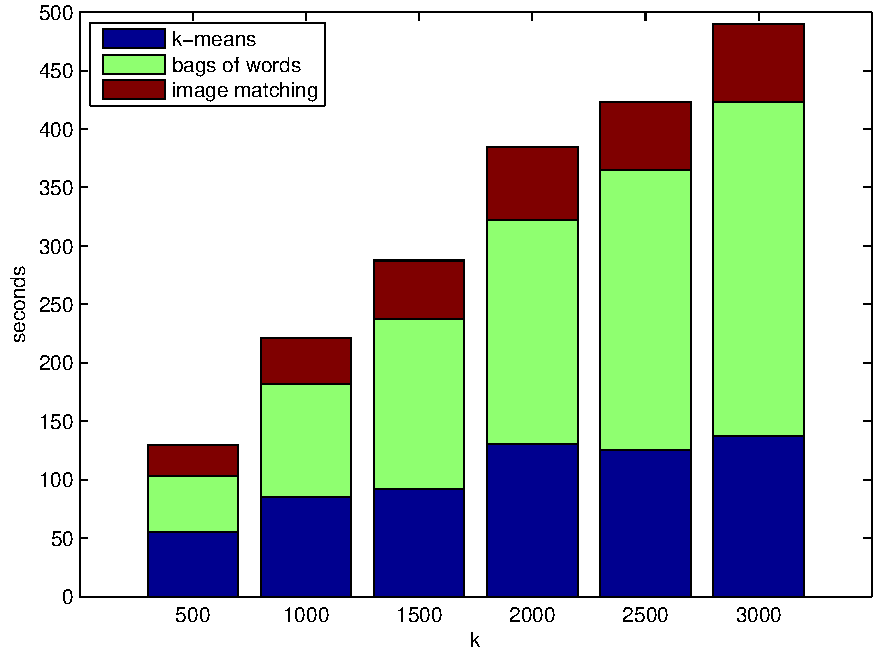
\includegraphics[width=\textwidth]{images/results_k_time.pdf}
        \label{fig:results_k_time}
        \caption{Computation time for $n_{train} = 5$ and varying $k$.}
    \end{subfigure}
    \begin{subfigure}[t]{0.48\textwidth}
        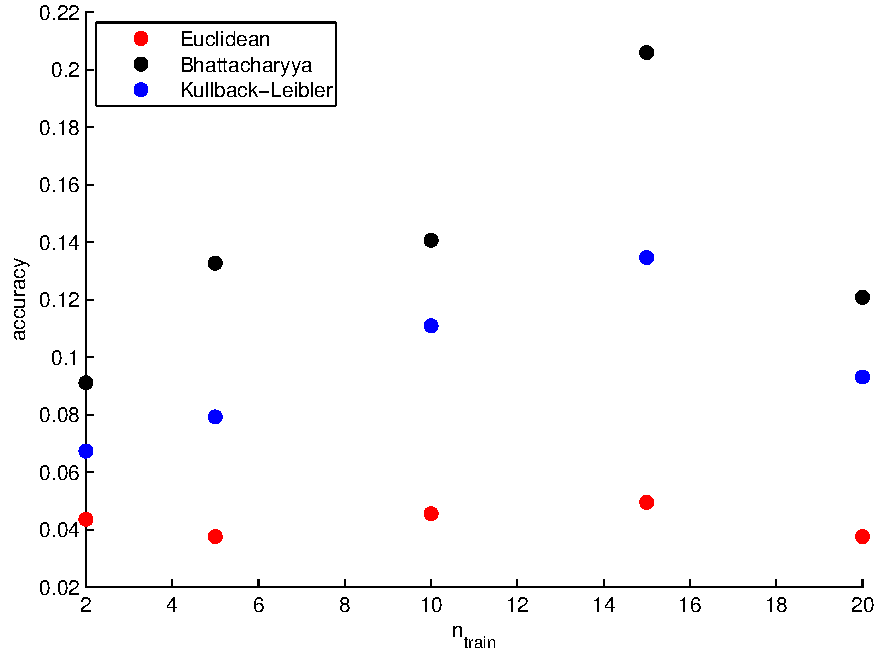
\includegraphics[width=\textwidth]{images/results_n_train.pdf}
        \label{fig:results_n_train}
        \caption{Matching accuracy for $k = 2500$ and varying $n_{train}$.}
    \end{subfigure}
    \begin{subfigure}[t]{0.48\textwidth}
        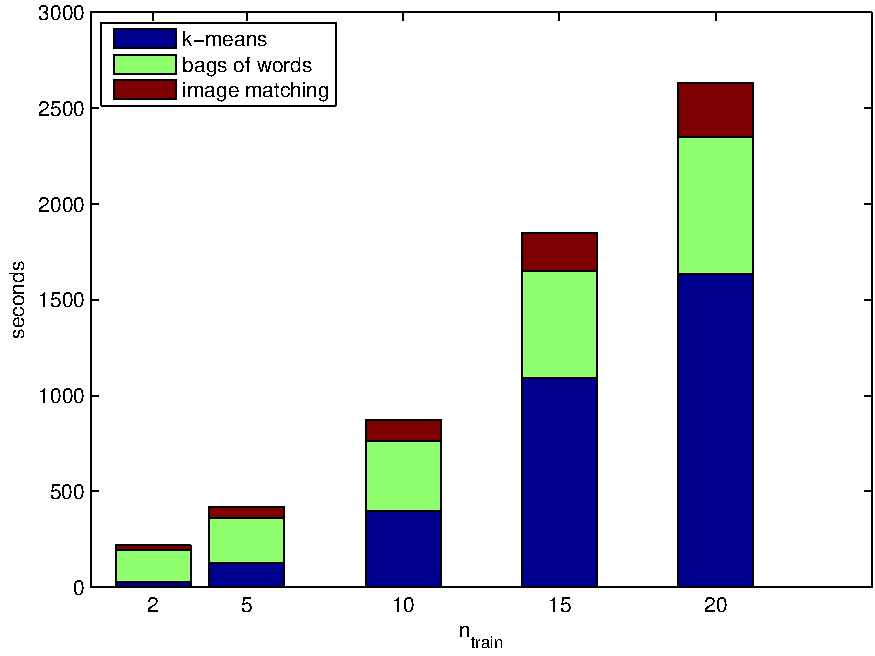
\includegraphics[width=\textwidth]{images/results_n_train_time.pdf}
        \label{fig:results_n_train_time}
        \caption{Computation time for $k = 2500$ and varying $n_{train}$.}
    \end{subfigure}
    \caption{Parameter study results for training and testing the
    implementation}
    \label{fig:parameter_results}
\end{figure}

\subsection{Examples of resulting retrieving}

\begin{figure}[H]
\centering
\adjincludegraphics[scale=.4]{images/results_11.pdf}
\label{fig:results_11}
\caption{Example of successful image matching: test image with its 3 best
    training image matches, along with their bag of words histograms.}
\end{figure}
%
\begin{figure}[H]
\centering
\adjincludegraphics[scale=.4]{images/results_18.pdf}
\label{fig:results_18}
\caption{Example of failed image matching: test image with its 3 best training
    image matches, along with their bag of words histograms.}
\end{figure}
%
\end{document}
